\svnid{$Id$}
\chapter{Discussion and Completed Model}
\label{chap:completedmodel}
%Therefore I have integrated microbiological techniques with mathematical modelling principles to allow us to understand the system in a way previously not possible. I have constructed a mathematical model which describes \Nsm{} respiration \textit{in silico} and can produce predictions for the system \textit{in vivo}. To parametrise this model I used a novel integrative scheme where a standard Bayesian fitting methodology is interleaved with iterative experimental data collection on progressively more complex respiratory scenarios.
From Chapter \ref{chap:intro}, the stated aims of this thesis were:
\begin{enumerate}
\item {\bf Construct a mathematical model of the \Nm{} respiratory chain.} This will involve the conversion of the kinetic reactions involved in respiration into mathematical equations that can be linked together, and if justified simplifying the chain.
\item {\bf Obtain experimental data on respiratory rates and enzyme kinetics.} This will involve performing experiments on respiring \Nm{} and recording the concentrations of respiratory substrates under different conditions.
\item {\bf Parametrise the model using experimental data.} To do this a system will need to be developed which can iteratively fit experimental data to specific parts of the mathematical model.
\end{enumerate}

\noindent With reference to the above, the a mathematical model was constructed as described in Chapter \ref{chap:model}, the equations shown below:
\begin{eqnarray*}
\frac{d[O_2]}{dt} & = & \beta(1-[O_2]/K_O) - k_{1}[C_a][O_2]\\ \nonumber
\frac{d[NO]}{dt} & = & m_{1}[NO_2^-][A_a] - l_1[NO][B_a] - k_5[C_a][NO] + k_6 [C_X] - \gamma[NO]\\ \nonumber
\frac{d[NO_2^-]}{dt} & = & - m_{1}[NO_2^-][A_a]\\ \nonumber
\frac{d[Q_a]}{dt} & = & g([Q] - [Q_a]) - l_3[Q_a]([B] - [B_a]) - f[Q_a]([X]-[X_a])\\ \nonumber
\frac{d[X_a]}{dt} & = & -k_3([C] - [C_a] - [C_X])[X_a]  - m_3([A] - [A_a])[X_a] + f[Q_a]([X]-[X_a])\\ \nonumber
\frac{d[C_a]}{dt} & = & k_3([C] - [C_a] - [C_X])[X_a] - k_{1}[C_a][O_2] - k_5[C_a][NO] + k_6[C_X]\\ \nonumber
\frac{d[C_X]}{dt} & = & k_5[C_a][NO] - k_6 [C_X]\\ \nonumber
\frac{d[A_a]}{dt} & = & m_3([A] - [A_a])[X_a]- m_{1}[NO_2^-][A_a]\\ \nonumber
\frac{d[B_a]}{dt} & = & l_3[Q_a]([B] - [B_a]) - l_1[NO][B_a]
\end{eqnarray*}
Additionally if the preliminary suggested expression equations are to be included this list is extended to include:
\begin{eqnarray*}
\frac{d[A]}{dt} & = & \left(R\left(1 - \frac{[O_2] + k_{10}[NO]}{[O_2] + k_{10}[NO] + k_{11}}\right) - S\left(1 - \frac{[NO]}{[NO] + k_{13}}\right)\right) - k_8[A] \nonumber \\
\frac{d[B]}{dt} & = & T \left(\frac{[NO]}{[NO] + k_{15}}\right) - k_{16}[B]
\end{eqnarray*}

The data required to populate the parameters has been obtained by experimental means as described in Chapters \ref{chap:oxygenreduction}-\ref{chap:nitritereduction}. These data provided information on both respiratory rates and enzymes kinetics. Additional information was gathered from the literature as shown in Chapter \ref{chap:model}.

To use the information obtained from the literature and from experimental data, an integrated parameter estimation scheme was devised, which combined Bayesian inference with a Monte-Carlo type parameter estimation system into an iterative method for extracting parameter values from progressively more complex datasets as described in Chapter \ref{chap:paramest}. This iterative method produces posterior probability distributions for each of the parameters in the model calculated from the various rounds of parameter estimation for each successive dataset. The final parameter probability distributions are shown in tabular form in Table \ref{tab:final_parameters}. This table shows the values required to produce idealised lognormal distributions of each of the parameters. Plots of the actual obtained distributions are shown in Figure \ref{fig:final_posteriors}.
\begin{table}[tbp]
\begin{center}
\begin{tabular}{>{\centering}m{1.4cm}>{\centering}m{6.1cm}>{\centering}m{2.7cm}>{\centering}m{2.5cm}}
\toprule
\textbf{Symbol} & \textbf{Description} & \textbf{Mean Value} & \textbf{$\sigma$}
\tabularnewline
\midrule
$k_1$ & Rate constant for O$_{\textrm{2}}$ reduction by reduced \cbbthree{} & $403.51~\mu M^{-1} s^{-1}$ & $27.59$
\tabularnewline\noalign{\smallskip}\hline\noalign{\smallskip}

$k_3$ & Rate constant for \cbbthree{} reduction by cytochrome pool & $4.58~\mu M^{-1} s^{-1}$ & $0.436$
\tabularnewline\noalign{\smallskip}\hline\noalign{\smallskip}

$l_1$ & Rate constant for NO reduction by reduced NorB & $6.42~\mu M^{-1} s^{-1}$ & 2.33
\tabularnewline\noalign{\smallskip}\hline\noalign{\smallskip}

$l_3$ & Rate constant for NorB reduction by quinone pool & $0.096~\mu M^{-1} s^{-1}$ & $0.025$
\tabularnewline\noalign{\smallskip}\hline\noalign{\smallskip}

$m_1$ & Rate constant for NO$_{\textrm{2}}^{\textrm{-}}$ reduction by reduced AniA & $0.175~\mu M^{-1} s^{-1}$ & $0.087$
\tabularnewline\noalign{\smallskip}\hline\noalign{\smallskip}

$m_3$ & Rate constant for AniA reduction by cytochrome pool & $4.79~\mu M^{-1}s^{-1}$ & $0.042$
\tabularnewline\noalign{\smallskip}\hline\noalign{\smallskip}

$k_5$ & Rate constant for \cbbthree{} inhibition by NO & $\approx66000~\mu M ^{-1} s ^{-1}$ & Indeterminate
\tabularnewline\noalign{\smallskip}\hline\noalign{\smallskip}

$k_6$ & Rate constant for recovery of NO inhibited \cbbthree{} & $1.59~s^{-1}$ & $0.527$
\tabularnewline\noalign{\smallskip}\hline\noalign{\smallskip}

$\beta$ & Rate constant for passive diffusion in of O$_{\textrm{2}}$ & $0.00014~\mu M^{-1} s^{-1}$ & $4.7\times10^6$
\tabularnewline\noalign{\smallskip}\hline\noalign{\smallskip}

$K_O$ & Saturation O$_{\textrm{2}}$ level & $48~\mu M$ & $0$
\tabularnewline\noalign{\smallskip}\hline\noalign{\smallskip}

$g$ & Rate of electrons in from NADH & $0.085~s^{-1}$ & $0.0078$
\tabularnewline\noalign{\smallskip}\hline\noalign{\smallskip}

$f$ & Rate constant for reduction of cytochromes by quinones & $0.771~\mu M^{-1}s^{-1}$ & $0.096$
\tabularnewline\noalign{\smallskip}\hline\noalign{\smallskip}

$\gamma$ & Spontaneous loss of NO & $0.0024~\mu Ms^{-1}$ & $8.8\times10^5$
\tabularnewline\noalign{\smallskip}\hline\noalign{\smallskip}

$Q$ & Concentration of quinones & $34.31~\mu M$ & $5.49$
\tabularnewline\noalign{\smallskip}\hline\noalign{\smallskip}

$X$ & Concentration of cytochromes & $2.81~\mu M$ & $0.595$
\tabularnewline\noalign{\smallskip}\hline\noalign{\smallskip}

$A$ & Concentration of AniA & $0.704~\mu M$ & $0.3$
\tabularnewline\noalign{\smallskip}\hline\noalign{\smallskip}

$B$ & Concentration of NorB & $7.8~\mu M$ & $3.63$
\tabularnewline\noalign{\smallskip}\hline\noalign{\smallskip}

$C$ & Concentration of \cbbthree{} & $1.3~\mu M$ & $0.259$
\tabularnewline
\bottomrule
\end{tabular}
\caption[Model parameters]{{\bf Model parameters.} This table shows all the parameter values that have been generated by iterative parameter estimation throughout this work. For values that show concentrations of components, they represent the value for a culture with $OD_{600}=1.00$.
\label{tab:final_parameters}}
\end{center}
\end{table}

\begin{figure}[tbp]
 \centering
 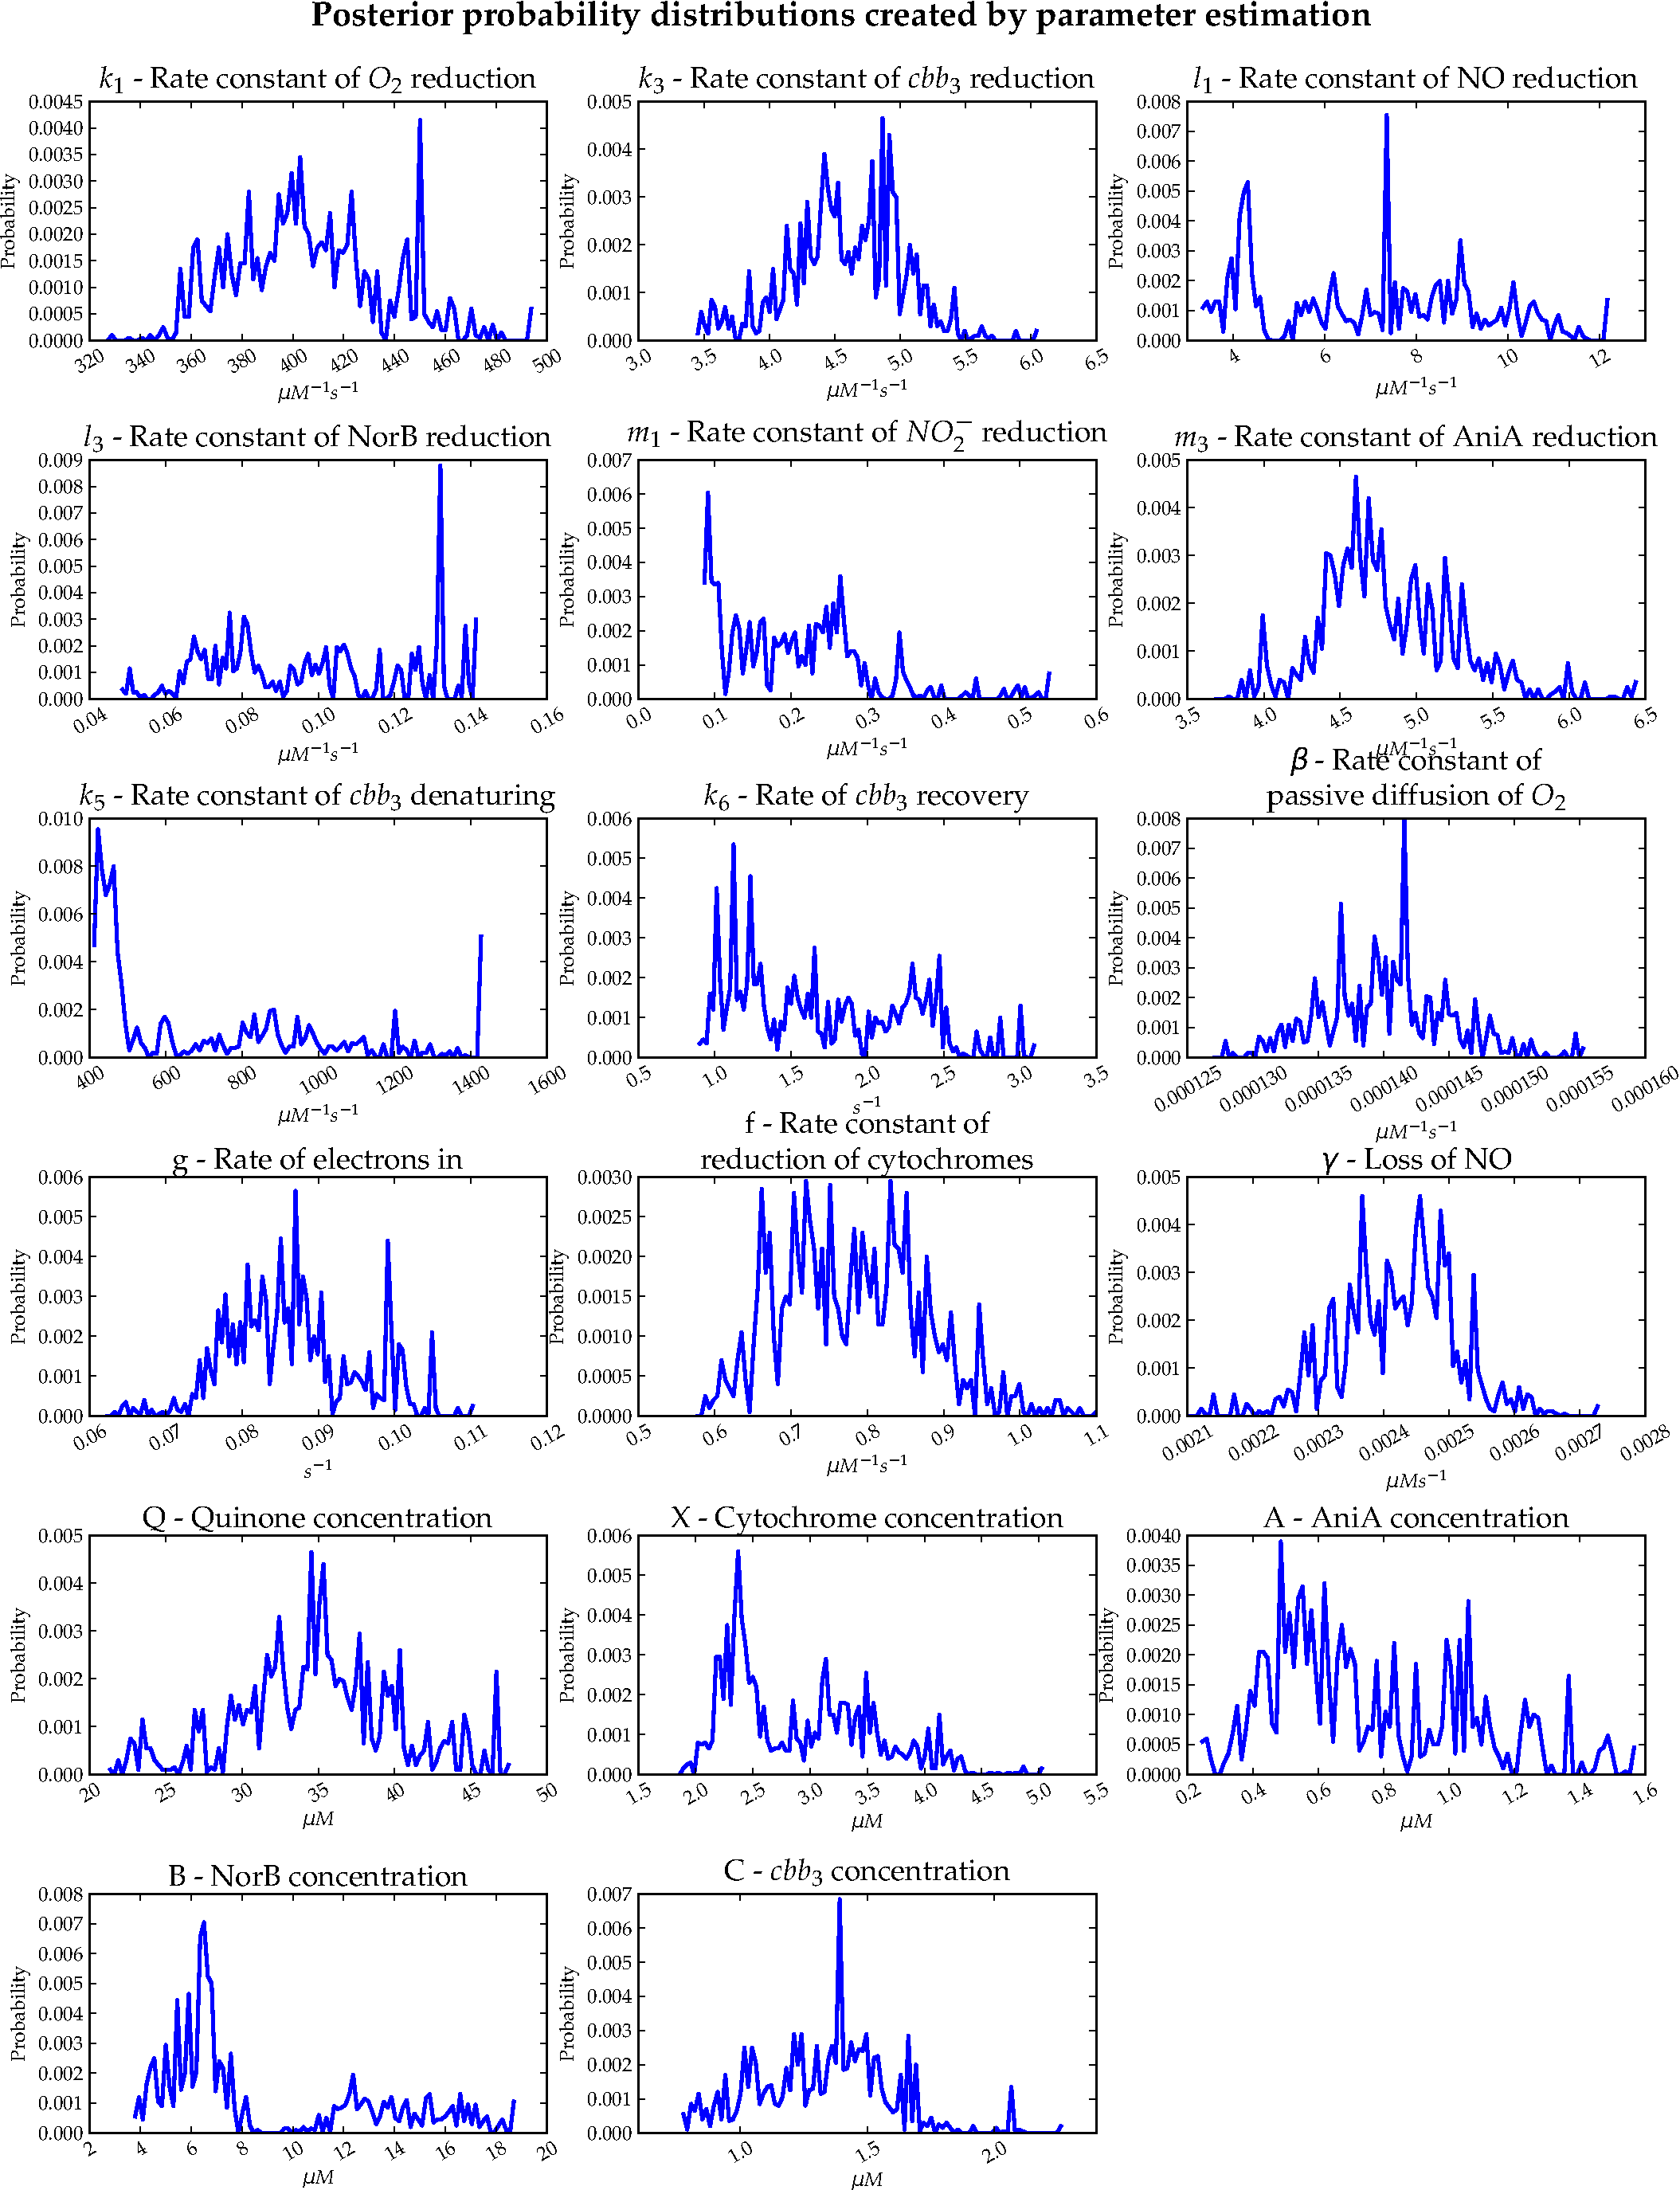
\includegraphics[width=15cm, trim=0cm 0cm 0cm 0cm, clip=true]{./09-completedmodel/data/posteriors.pdf}
 % priors.pdf: 1008x1008 pixel, 72dpi, 35.56x35.56 cm, bb=0 0 1008 1008
 \caption[Final Posterior probability distributions]{{\bf Final Posterior probability distributions}. These are the final posterior probability distributions generated by the parameter estimation system, all concentrations have been normalised to assume an $OD_{600}$ of 1. Note the value of $k_5$ will be significantly different from that shown.
 \label{fig:final_posteriors}}
\end{figure}

The value of $k_5$ has no associated bounds in the table as it was concluded that the value reported is actually much lower than the true value as evidenced in Chapter \ref{chap:nitritereduction} whereby the posterior parameters from nitrite reduction were unable to model the true effect of NO inhibition of oxygen shown in Chapter \ref{chap:noreduction}. Increasing the value of $k_5$ could restore the correct behaviour in the NO reduction dataset without a significant detrimental effect on the nitrite dataset. Unfortunately this makes the bounds on this value indeterminate without further Monte-Carlo simulation being run with the adapted value. The distribution shown in Figure \ref{fig:final_posteriors} shows the un-adapted values for comparison.

\section{Amalgamation of Cytochromes}
The choice to replace the multiple cytochromes $bc_1$, $c_x$, $c_4$ and $c_5$ with one single entity was a modelling one, to both simplify the modelling process by reducing the total component count and number of rate constants, and to allow the model to focus on simple electron transport chain branching and competition for electrons. The rate constants for each of the cytochromes could be subsumed by the respective ``out rates'' from the amalgamated cytochrome to its downstream electron acceptor. The downside of this approach is that it means that any rates obtained for $X$ are probably not going to be biologically relevant as it is essentially masking the behaviour of multiple different hidden components. This simplification does not appear to have affected the model in a detrimental way when using the datasets in this work.

\section{Concluding Remarks}
The parametrised model created in this work appears to be capable of at least qualitatively modelling the behaviour of all the datasets presented, using the final set of parameter distributions. The model is not 100\% qualitative, although this was not an implicit requirement for the model. It should still be capable of offering insight into how the system behaves even if it cannot predict changes precisely. The non-quantitative nature of the model was to be expected given the high level of complexity in the model and some of the assumptions made regarding cytochromes, backward reaction rates etc. The most obvious ``fault'' in the model is that there is an incomplete decoupling of cell density from other components. Unfortunately this is most probably because the proxy used was not completely accurate as a replacement for cell density.

The integrated parameter estimation system created for this work operates as intended and could be extended to parametrise other systems if the same Bayesian approach were taken to data gathering. It is not however a system that could be used without human curation though, as it can still produce mathematically correct results with parameters that are actually very unlikely \textit{in vivo}. This was shown in Chapter \ref{chap:nitritereduction} where the values for 2 parameters were an order of magnitude too high in the prior probability distributions causing the simulation to fail. These same values worked ``perfectly'' for the datasets in Chapters \ref{chap:oxygenreduction} and \ref{chap:noreduction}. Such human interaction with the system is important however as it forms part of the Bayesian approach whereby we provide the ``prior'' knowledge to the system.

In conclusion, a novel system for parametrising a respiration system model has been created and utilised which has been able to successfully populate the model and produce probability distributions for all parameters. These parameters are able to be used in a qualitative manner to match existing experimental data, and to provide insight into the hidden behaviour of the system.